\documentclass{article}
\usepackage[utf8]{inputenc}
\usepackage{fullpage}
\usepackage{graphicx}
\usepackage{amsmath}
\usepackage{enumitem,amssymb}
\newlist{todolist}{itemize}{2}
\setlist[todolist]{label=$\square$}
\usepackage{pifont}
\newcommand{\cmark}{\ding{51}}%
\newcommand{\xmark}{\ding{55}}%
\newcommand{\done}{\rlap{$\square$}{\raisebox{2pt}{\large\hspace{1pt}\cmark}}%
\hspace{-2.5pt}}



\title{TheLastDance}
\author{Kasper Verhulst}
\date{February 2021}

\begin{document}

\begin{table}[h]
\def\arraystretch{1.8}
\begin{tabular}{|llll|}
\hline
\multicolumn{4}{|c|}{\Large \textbf{The Last Dance}}                                                                                         \\ \hline

\multicolumn{2}{|p{0.4\textwidth}|}{Organization: HackTheBox}     &    \multicolumn{2}{|l|}{Type: offline challenge}    \\ \hline
\multicolumn{3}{|l|}{
    \begin{minipage} [t] {0.07\textwidth} 
Categories:
    \end{minipage} 
    \begin{minipage} [t] {0.3\textwidth} 
      \begin{itemize}
        \begin{todolist}
            \item Network Security
            \item[\done] Cryptography
            \item Mobile Applications
        \end{todolist}
     \end{itemize} 
    \end{minipage} 
     \begin{minipage} [t] {0.3\textwidth} 
      \begin{itemize}
         \begin{todolist}
            \item Reverse Engineering
            \item Web Applications
            \item Forensics
         \end{todolist}
        \end{itemize} 
    \end{minipage} 
    } & \multicolumn{1}{|l|}{Difficulty: Easy} \\ \hline
     \multicolumn{2}{|l|}{Name: Kasper Verhulst} & \multicolumn{2}{|l|}{\begin{tabular}[c]{@{}r@{}}Release date: 23-05-2020\\ Completing date: 28-12-2022\end{tabular}} \\ \hline
\end{tabular}
\end{table}

\section*{Understanding the challenge}
The challenge brings an encryption script and the some file containing the output of a round of such encryption. The encryption function will start by generating a random key and nonce. These two values will be used to initialize a ChaCha20 cipher. Afterwards, a hard-coded message and the flag are individually encrypted using the same instance of the ChaCha20 encryption machine. 

\section*{Stream Ciphers}
ChaCha20 is an alternative to AES adopted by the TLS-standard. Contrarily to AES, ChaCha is a stream cipher. Fundamentally all stream ciphers follow the same idea. A key generation function is used to extend a key together with an initial value to a pseudorandom, continuous output. Afterwards, the plaintext is XORed with this key stream. Decryption happens exactly the same way. Since stream cipher are still symmetric encryption mechanism, the receiver will have access to the shared key. He can recreate the key stream and xor the ciphertext to obtain the original plaintext. Figure \ref{fig:stream} illustrates stream ciphers.

\begin{figure}[h]
    \centering
    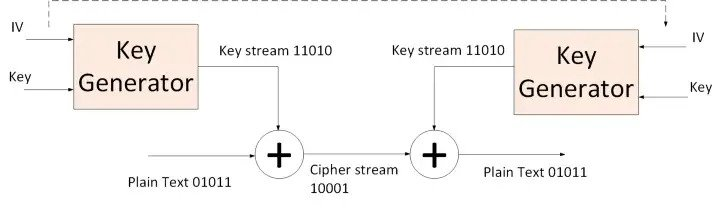
\includegraphics[width=0.99\textwidth]{streamcipher.jpg}
    \caption{Stream cipher}
    \label{fig:stream}
\end{figure}

\begin{equation}
\begin{split}
    K &= PRF(key,IV) \\
    C_i &= K_i \oplus P_i \\ 
\end{split}
\end{equation}

\section*{Solving the challenge}
Once we understand how stream ciphers work, it is clear that key reuse is completely breaking the security of a stream cipher. The encoded file contains two encrypted messages that we can use:

\begin{equation}
\begin{split}
    C_1 &= ChaCha_1(key,IV) \oplus P_1 \\  \\
    C_2 &= ChaCha_2(key,IV) \oplus P_2 \\ 
\end{split}
\end{equation}
Combining bot equations,
\begin{equation}
    C_1 \oplus C_2 = (ChaCha_1(key,IV)) \oplus P_1 \oplus ChaCha_2(key,IV) \oplus P_2 )
\end{equation}

Since the same key and initialization vector were used:

\begin{equation}
    C_1 \oplus C_2 = k \oplus P_1 \oplus k \oplus P_2 )
\end{equation}

\begin{equation}
    C_1 \oplus C_2 =   P_1 \oplus P_2
\end{equation}
Since we have both ciphertexts, and we know the hard-coded message that was also encrypted:

\begin{equation}
    C_2 =   P_1 \oplus P_2 \oplus C_1
\end{equation}

\end{document}
